\section{Simulation}
In a 2D region, points with the same TDOA to two fixed locations form a hyperbola. However, in practical systems, we can only measure TDOA up to a precision.Therefore we look at all points with difference of distance close to some target value within measurement error $\epsilon$. This $\epsilon$ prepresents accuracy on measurement of difference of distances, and in practice it is related to sampling rate and TDOA methods.

\begin{figure}[]
  \centering
  \begin{subfigure}[]{.23\textwidth}
    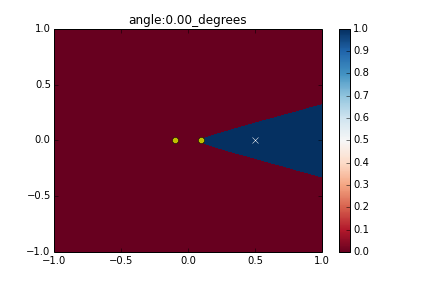
\includegraphics[width=\textwidth]{sim/sim_2_1}
    \caption{micro-controller}
  \end{subfigure}
  \begin{subfigure}[]{.23\textwidth}
    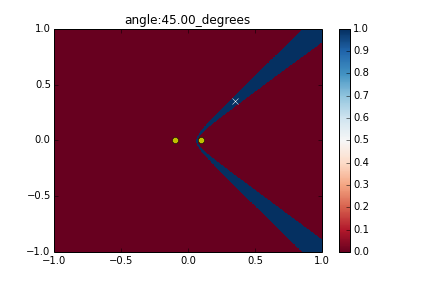
\includegraphics[width=\textwidth]{sim/sim_2_2}
    \caption{array}
  \end{subfigure}
  \begin{subfigure}[]{.23\textwidth}
    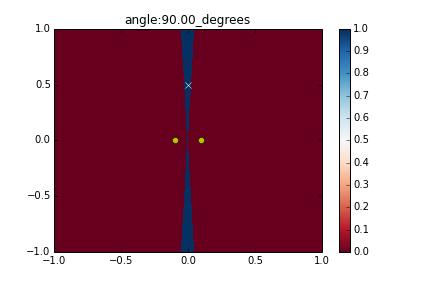
\includegraphics[width=\textwidth]{sim/sim_2_3}
    \caption{two arrays}
  \end{subfigure}
  \caption{Localization arrays}
  \label{fig:sim_2_5}
\end{figure}

To see how precision affects localization accuracy, we simulated two microphones placed at: $M_1:(x=-10\mbox{cm},y=0\mbox{cm})$ and $M_2:(x=10\mbox{cm},y=0\mbox{cm})$. A test sound source is emitted at point $P$ $50$ centimeters away from $(0,0)$. Fig~\ref{fig:sim_2_5} shows the region where all points $\hat P$ satisfy:
\[
 |(\hat P M_1 - \hat P M_2) - (P M_1 - P M_2)| < 1 \mbox{cm}
\]
Intuitively, points in the region have difference of distance very similar to each other. From fig~\ref{fig:sim_2_5}, the region still has the shape of a hyperbola, but with an uncertainty region around the curvce. The uncertainty region is not uniform around the curve, the farther away the point is, the larger the uncertainty region becomes. It indicates that the samve delta distance movement will generate smaller difference of distance when you are farther away from the array. The size of the uncertianty region is also angle dependent: points closer to the line of microphones have larger region compared to points close to the line perpenticular to microphones. 

\begin{figure*}[]
  \centering
  \begin{subfigure}[]{.3\textwidth}
    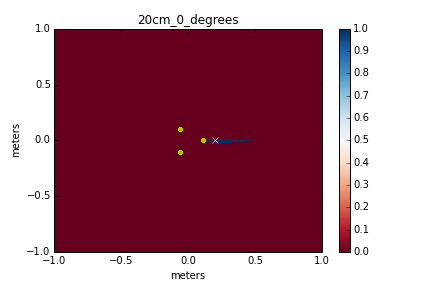
\includegraphics[width=\textwidth]{sim/result_20cm_0_degrees}
    \caption{0 degrees}
  \end{subfigure}
  \begin{subfigure}[]{.3\textwidth}
    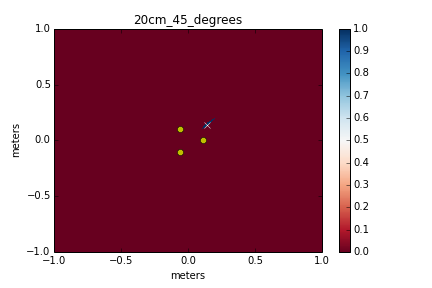
\includegraphics[width=\textwidth]{sim/result_20cm_45_degrees}
    \caption{45 degrees}
  \end{subfigure}
  \begin{subfigure}[]{.3\textwidth}
    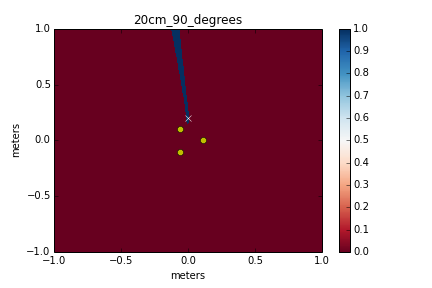
\includegraphics[width=\textwidth]{sim/result_20cm_90_degrees}
    \caption{90 degrees}
  \end{subfigure}
  \begin{subfigure}[]{.3\textwidth}
    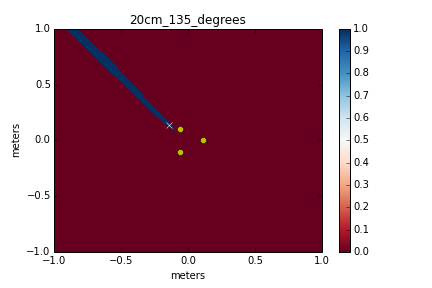
\includegraphics[width=\textwidth]{sim/result_20cm_135_degrees}
    \caption{135 degrees}
  \end{subfigure}
  \begin{subfigure}[]{.3\textwidth}
    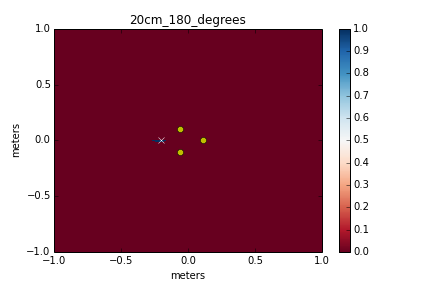
\includegraphics[width=\textwidth]{sim/result_20cm_180_degrees}
    \caption{180 degrees}
  \end{subfigure}
  \caption{$20$cm equilateral triangle array. Source is $20$cm away from the array}
  \label{fig:sim_3_2}
\end{figure*}

\begin{figure*}[]
  \centering
  \begin{subfigure}[]{.3\textwidth}
    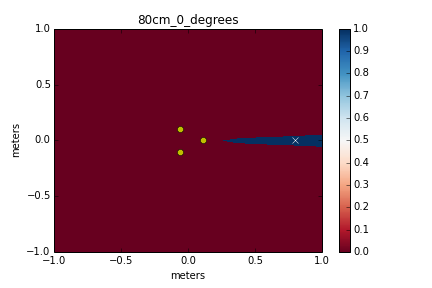
\includegraphics[width=\textwidth]{sim/result_80cm_0_degrees}
    \caption{0 degrees}
  \end{subfigure}
  \begin{subfigure}[]{.3\textwidth}
    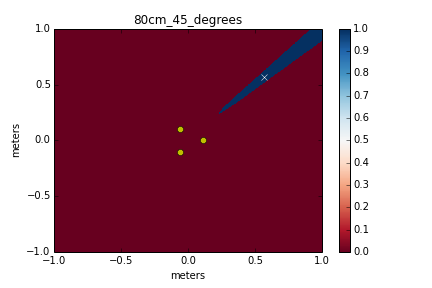
\includegraphics[width=\textwidth]{sim/result_80cm_45_degrees}
    \caption{45 degrees}
  \end{subfigure}
  \begin{subfigure}[]{.3\textwidth}
    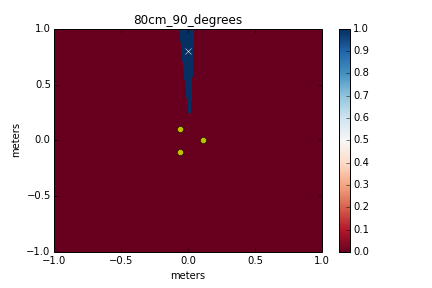
\includegraphics[width=\textwidth]{sim/result_80cm_90_degrees}
    \caption{90 degrees}
  \end{subfigure}
  \begin{subfigure}[]{.3\textwidth}
    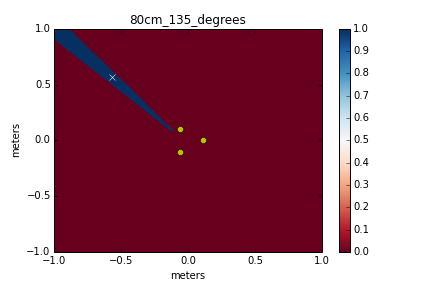
\includegraphics[width=\textwidth]{sim/result_80cm_135_degrees}
    \caption{135 degrees}
  \end{subfigure}
  \begin{subfigure}[]{.3\textwidth}
    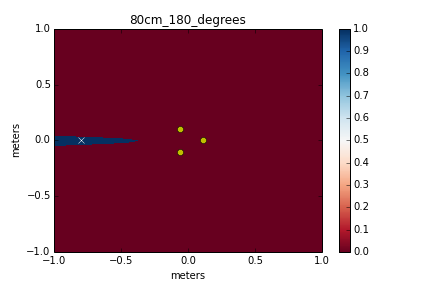
\includegraphics[width=\textwidth]{sim/result_80cm_180_degrees}
    \caption{180 degrees}
  \end{subfigure}
  \caption{$20$cm equilateral triangle array. Source is $80$cm away from the array}
  \label{fig:sim_3_8}
\end{figure*}

With more than two multiple microphones, each pair of microphones generates a hyperbolic region and localization becomes finding the intersection of regions. The smaller the intersection region, the better the localization accuracy. To see how accuracy changes with array placement and sound source location, three microphones are placed at three vertices of an $20$cm equilateral triangle. An audio source is placed at $20$ cm away from the center of the array. Fig~\ref{fig:sim_3_2} shows the intersection of regions for $5$ different placement of the sound source. It can be seen that accuracy is worse when sound source is close to the line of any two microphones. This observation is consistent with two microphone case, since points close to line of microphones have a larger uncertainty region.

To see how sound source distance affects localization accuracy, the same simulation is carried out with sound source moved from $20$cm to $80$cm away from the center of the array. Results are presetned in fig~\ref{fig:sim_3_8}. Comparing with fig~\ref{fig:sim_3_2}, accuracy decreases with distance to the array. This is also consistent with our observation in $2$ microphone case where source farther away would result in larger uncertainty region.

\begin{figure*}[]
  \centering
  \begin{subfigure}[]{.3\textwidth}
    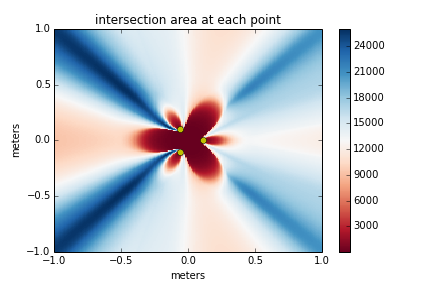
\includegraphics[width=\textwidth]{sim/result_intersection_area_at_each_point_3_center}
    \caption{$3$ microphones placed at vertices of an $20$cm equilateral triangle}
    \label{fig:sim_hm_3}
  \end{subfigure}
  \begin{subfigure}[]{.3\textwidth}
    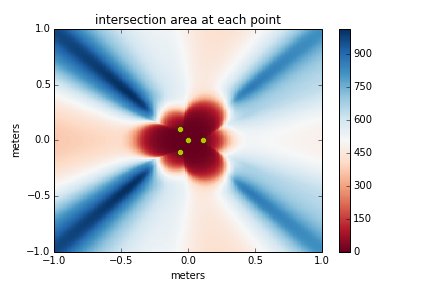
\includegraphics[width=\textwidth]{sim/result_intersection_area_at_each_point_3_p1}
    \caption{another microphone added at origin}
    \label{fig:sim_hm_3_p1}
  \end{subfigure}
  \begin{subfigure}[]{.3\textwidth}
    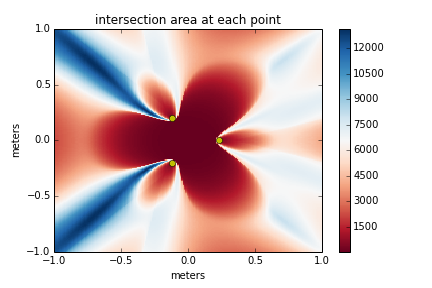
\includegraphics[width=\textwidth]{sim/result_intersection_area_at_each_point_3_2x}
    \caption{$3$ microphones placed at vertices of an $40$cm equilateral triangle}
    \label{fig:sim_hm_3_2x}
  \end{subfigure}
  \begin{subfigure}[]{.3\textwidth}
    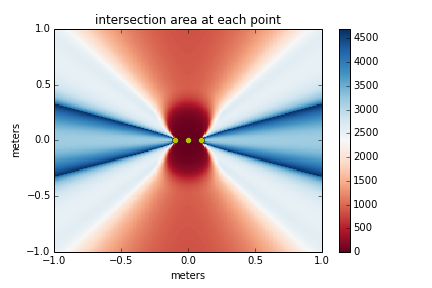
\includegraphics[width=\textwidth]{sim/result_intersection_area_at_each_point_3_line}
    \caption{$3$ microphones placed in a line. Total length is $20$cm}
    \label{fig:sim_hm_3_line}
  \end{subfigure}
  \begin{subfigure}[]{.3\textwidth}
    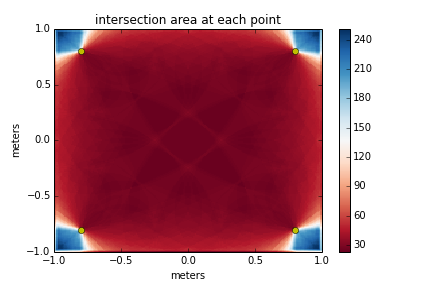
\includegraphics[width=\textwidth]{sim/result_intersection_area_at_each_point_4corner}
    \caption{$4$ microphones placed at $4$ corners of the region}
    \label{fig:sim_hm_4}
  \end{subfigure}
  \begin{subfigure}[]{.3\textwidth}
    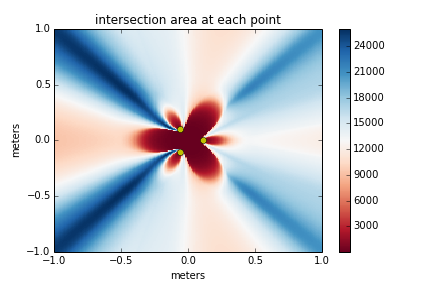
\includegraphics[width=\textwidth]{sim/result_intersection_area_at_each_point_3_center}
    \caption{two $3$ microphone arrays placed $1$ meter apart}
    \label{fig:sim_hm_2_array}
  \end{subfigure}
  \caption{Accuracy for different array configurations}
  \label{fig:sim_hm}
\end{figure*}

Intersection area is a measure of the localization accuracy. To evaluate an array's accuracy in a region, we can place sound source at predetermined grid points in the region and look at the intersection area for each point in the grid. Results for a few different configurations are presented in fig~\ref{fig:sim_hm}.

Fig~\ref{fig:sim_hm_3} shows the accuracy when microphones are placed at three vertices of an $20$ cm equilateral triangle. The region inside the array has good accuracy. However, for regions along line of any two microphones, the accuracy drops significantly. 

To evaluate how adding one microphone(without increasing array size) improves accuracy,  another microphone is added to the array at $(0,0)$. Result is presented in fig~\ref{fig:sim_hm_3_p1}. Addition of the new microphone only slightly improved the accuracy around the array region. Regions near lines of microphones still have significantly larger uncertainty region.

To evaluate array size's impact on accuracy, the size of original array from fig~\ref{fig:sim_hm_3} is increased by a factor of $2$. The result is presented in fig~\ref{fig:sim_hm_3_2x}. The overall uncertainty area decreased across the region. 

In fig~\ref{fig:sim_hm_3_line}, three microphones $10$cm apart from each other are placed in a line on x-axis. The result indicates that this configuration has high uncertainty in nearly all regions except for regions near the microphones. In fig~\ref{fig:sim_hm_4}, four microphones are placed at four corners of the region. Accuracy is consistently good across the region. However, this configuration requires microphone to be placed far apart.

To get benefit of far away microphone placement without incurring overhead of placing individual microphones, two array solutions are explored. Fig~\ref{fig:sim_hm_2_array} shows the accuracy map when two $3$ microphone array are placed $1$ meter apart.  It shows that the array has good accuracy inside a one meter by one meter region
